\chapter{Next Generation Flow Monitoring}\label{chap:next-generation-flow}

\begin{chapintro}

The work presented in this thesis so far aimed to improve the state of flow monitoring. We focused on including more information in flow records and on accelerating the flow monitoring for high-speed networks. The flow creation process and the structure of flow records adhered to the definitions provided in Chapters~\ref{chap:network-flow-monitoring} and~\ref{chap:application-flow-monitoring}. The goal of this chapter is to show how the flow monitoring might evolve in the future.

We present three novel concepts that might be applied to flow monitoring to increase the amount of information carried by the flow records. All concepts require adaptation of flow data processing to a certain degree as well. Moreover, the definitions of flows given in this thesis no longer hold for these novel concepts.

The first proposed concept is called EventFlow and is based on the assumption that each user action involving the use of network usually generates more than one flow. For example, simple access to a web page might create a DNS query and an HTTP query as well. The main goal of EventFlow is to connect the flows that are part of a single action or event. We have implemented a prototype for measurement of EventFlow and provide its evaluation in this chapter.

The second concept addresses the monitoring of tunnelled traffic. Currently, each flow that represents a tunnel is split into multiple flows based on the communication in that tunnel. However, this approach usually supports only a static number of encapsulation layers. We propose another approach based on a hierarchical tree of flows.

Similarly to the monitoring of tunnelled traffic, application events can also cause a flow to be split into several smaller flows. This causes statistics relying on a number of flows as well as per-flow metrics to be inaccurate. The last concept proposes to handle application layer events separately from flow records. Each event would be associated with the original flow, however, would not influence its creation at all.

The paper included in this chapter is~\cite{Velan-2016-EventFlow}.

The organisation of this chapter is as follows:
\begin{itemize}
  \item Section~\ref{sec:eventflow} describes the design and evaluation of the EventFlow concept.
  \item Section~\ref{sec:metaflow} presents and discusses the MetaFlow concept.
  \item Section~\ref{sec:app-events} introduces the concept of application events in flow.
  \item Section~\ref{sec:ng-summary} summarizes the chapter.
\end{itemize}

\end{chapintro}

\newpage

\section{EventFlow}\label{sec:eventflow}

%% motivation
Application flow monitoring parses data from application headers and adds application-specific elements to flow records. This way the information from application level can be easily transferred to flow collectors, stored, and utilised together with the information about the network communication. The current approach is to treat separate application protocols individually, e.g., develop an application processing module for each monitored protocol, as shown in Chapter~\ref{chap:application-flow-monitoring}. However, connections between different protocols are lost in this scenario. For example, when a user wants to access a web page, several different flows records are created. The DNS server must be contacted to resolve the hostname of the web page to an IP address. After the basic document is loaded, the user's browser automatically loads linked content, such as images, cascading style sheets, and javascript libraries. The generated requests are recorded as flows; however, only a little relation between the flows is preserved.

Information about relations between individual flows can be useful in several scenarios. First, when an advertisement on a web page contains malware, the page can be traced using the relation and notified of the malicious content. Second, aggregates of the related flows can be created to simplify behavioural analysis of network traffic. Moreover, the analysis can use the additional information to improve its accuracy. Last, traffic classification engines can also benefit from having access to information about flow relations~\cite{Wang-2014-Internet}.

%% goals
In this section, we present a flow monitoring extension, called EventFlow, which allows keeping track of relations between HTTP and DNS application flows. Information about flow relation is inserted to flow records to keep track of individual user actions, i.e., events. We develop a prototype of the EventFlow extension and evaluate its properties on network traffic trace from an ISP network. Results show that at least 10\,\% of HTTP and DNS flow records form complex events. We believe, that this is only a lower bound and that further improvements can be made to relate even more flows into events.

The rest of the section is structured as follows. Related work is surveyed in Subsection~\ref{subsec:eventflow-related_work}. We propose the architecture of EventFlow measurement in Section~\ref{subsec:eventflow-architecture}. Subsection~\ref{subsec:eventflow-prototype} describes the implementation of the EventFlow prototype. Experimental evaluation of the EventFlow prototype is performed in Subsection~\ref{subsec:eventflow-evaluation}. The section is concluded in Subsection~\ref{subsec:eventflow-conclusions}.


\subsection{Related Work} \label{subsec:eventflow-related_work}

Madhyastha and Krishnamurthy~\cite{Madhyastha-2008-Generic} propose a generic language for application-specific flow sampling. Their language allows applications to select flows with special properties so that the negative impact of sampling on these applications is minimised. This can be useful for intrusion detection systems or traffic classification applications. Although the goal of this work is different from ours, it also aims to improve the collected data, so that traffic analysis applications can achieve higher accuracy.
% language for app-specific flow sampling
% better flow sampling, applications can say what they need
% allows to select flows with special properties -> ease of processing for end applications such as IDS or traffic classification applications.

The authors of~\cite{Lee-2015-Flow} also focus on improving quality of sampled flow data. They show that the traffic classification accuracy can be increased using related sampling, which assigns a higher probability to connections that are part of the same application. The authors propose to use a source IP address as a measure of the relation between connection sessions.
% sampling based on flow relation - same IP address
% more flow per application session 
% better classification accuracy

Hu et al.~\cite{Hu-2009-Entropy} propose an entropy-based aggregation system to mitigate an impact of DoS attacks and worm spreads on a network monitoring system. The main contribution of their approach is a flow key attribute selection algorithm that chooses key attributes by which the flows are aggregated. A two-dimensional hash table is used to implement their approach. The aggregated flows are called metaflows. The main difference from EventFlow is that we label existing flows belonging to the same user action, while the metaflow is a substitute flow for many flows created during malicious network activity.
% aggregation to metaflows in case of DoS or worm spread
% the most important part is the selection of flows to aggregate and appropriate key attributes for the aggregation
% two-dimensional hash table

Dolberg et al.~\cite{Dolberg-2012-Efficient} introduce a multidimensional flow aggregation aimed to reduce the volume of collected data. The authors use tree structures for storing the data by chosen dimension such as IP addresses or ports. EventFlow proposed in our work might be used in this scenario to aggregate flows by the same events.
% multi-dimensional aggregation of stored information
% reducing the amount of data
% using tree structures
% has a few relevant aggregation citations

% Removed due to the lack of space
The usual approach to reducing the volume of collected data is to use sampling. Estan et al.~\cite{Estan-2004-Building} propose to use adaptive sampling rate to achieve highest possible accuracy within given data collection constraints. Their main contribution is a system for renormalisation of flow entries after the sampling rate was changed. The authors propose an extension to standard flow counting that increases the accuracy of the counters for sampled flow.
% adaptive sampling rate
% renormalisation of flow entries after sampling rate change by manipulating packet and byte counters in existing entries


\subsection{EventFlow Architecture} \label{subsec:eventflow-architecture}

This section describes the architecture of the EventFlow monitoring. The goal is to label all flows that are the results of a single user action with the same event identifier (EID). For example, accessing \url{http://www.w3.org/} creates 1 DNS request, 37 HTTP requests, and 8 HTTPS requests. We aim to assign a single unique EID to the flows generated for all these DNS and HTTP requests.

\begin{figure}[!tb]
    \centering 
    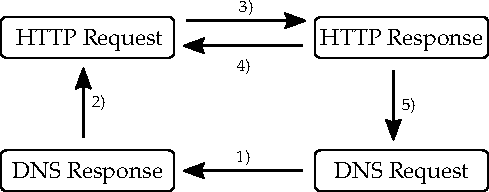
\includegraphics{figures/paper-eventflow/dependencies}
    \caption{Relations between HTTP and DNS Requests and Responses.}
    \label{fig:eventflow-relations}
\end{figure}

Four basic types of flows are recognised by the EventFlow: HTTP requests, HTTP responses, DNS requests and DNS responses. There are relations between these types of flows in network traffic, as shown in Figure~\ref{fig:eventflow-relations}. When HTTP request to a new site is performed, the IP address of the site must be resolved first. Therefore, a DNS request is created. After the request is observed, a reply usually follows, which results in the relation 1). After the DNS reply arrives, the client knows the IP address of the server and makes the HTTP request, which creates the relation 2). An HTTP response follows the request, as indicated by the relation 3). The HTTP response can contain an HTML page which links to several additional resources such as external style sheets or images. The loading of these resources triggers more HTTP requests, resulting in relation 4). When these requests point to previously unresolved domains, new DNS requests are created, which introduces the relation 5).

We base the EventFlow architecture on the relations between the requests and responses. When an HTTP or a DNS flow is encountered, we must make sure that it is assigned the same EID as the related flows. Therefore, we create four sets of records: expected HTTP requests, expected HTTP responses, expected DNS requests and expected DNS responses. When processing an HTTP or a DNS flow, we add a new record to the set or sets it relates to. Then, when a next flow is processed, it is matched against appropriate expected set to see whether it is a part of existing event. If it is, an EID of the event is assigned to the flow record. For example, when a DNS response is encountered, a new record is put into the expected HTTP requests set (because of relation 2), see Figure~\ref{fig:eventflow-relations}). Then, when an HTTP request is processed, we check the expected HTTP requests set to see whether we are expecting this request based on a previous DNS response. If the request is matched, it is assigned the same EID as the DNS response. 

\begin{table}[!t]
        \caption{Matched Flow Properties.}
        \centering
        \renewcommand{\arraystretch}{1.1}
        \begin{tabular}{l|c|c|c|c|c|c}
                         & \rotatebox[origin=r]{90}{\centering \textbf{Source IP}\hspace{33pt}} 
                         & \rotatebox[origin=r]{90}{\centering \textbf{Destination IP}\hspace{19pt}} 
                         & \rotatebox[origin=r]{90}{\centering \textbf{Destination Port}\hspace{9pt}} 
                         & \rotatebox[origin=r]{90}{\centering \textbf{URL}\hspace{48pt}} 
                         & \rotatebox[origin=r]{90}{\centering \textbf{Domain}\hspace{39pt}} 
                         & \rotatebox[origin=r]{90}{\centering \hspace{3pt}\textbf{DNS Transaction ID}} \\ \toprule
                        Expected HTTP Request  & \cmark &  &  & \cmark & \cmark &  \\ \hline
                        Expected HTTP Reply    & \cmark & \cmark & \cmark &  &  &  \\ \hline
                        Expected DNS Request   & \cmark &  &  &  & \cmark &  \\ \hline
                        Expected DNS Reply     & \cmark & \cmark & \cmark &  &  & \cmark \\ \bottomrule
        \end{tabular}
        \label{tab:eventflow-matched-properties}
\end{table}

Each of the sets of expected records uses different flow properties to match a flow record. When matching an HTTP request flow against the expected HTTP requests set, the source IP address of the flow must match as well as the requested domain or the URL, if available. Checking the source IP address ensures that flows from different hosts are not combined into a single event. A domain name is checked for the records that were inserted in the set when DNS reply was encountered. In case an HTTP response caused the record to be inserted, the full URL is available, not only the domain name. Replies are checked based on IP addresses and destination port. Source port is not checked since the services are expected to run on standard, well-known ports. The DNS reply is also checked for transaction ID, which is a unique identifier tying the request and response. However, the DNSSEC extension is ignored and does not affect the EventFlow. Therefore, any malicious responses would still be part of an event. List of the used properties is provided in Table~\ref{tab:eventflow-matched-properties}.

Expiration of the records from the expected sets must be ensured. When a record from any of the expected sets is matched, it is removed. However, many inserted records will never be matched. For example, when a DNS request is made to accommodate a different service than HTTP, the expected HTTP request might never appear. We need to free such records from the sets eventually. A timeout is used to keep the expected sets from being congested by redundant records. A timestamp is assigned to each record upon insertion to a set. Then, records older than the timeout are removed each time the set is searched. The timeout should be as short as possible to avoid blending of several events. However, it should be at least as long as it takes to process the longest user action, which might be up to a couple of seconds in case of complicated queries to slow sites.

There are several caveats to our approach and some limitations of the architecture that should be addressed in the future. Our approach does not handle HTTP redirection codes; therefore the first request and the HTTP 3xx redirection response are assigned different EID than the subsequent request to the resource. This problem can be rectified simply by adding a handler for the HTTP 3xx redirection responses that will put a new record with the redirect URL to the expected HTTP requests set.

Another limitation of our approach is that the URLs are only extracted from HTML documents. However, modern websites often use a JavaScript code to request additional resources through the Ajax technique. Such requests cannot be easily matched to an event since it would require to reconstruct the complete web page and process the included JavaScript code, which is infeasible for the flow monitoring system.

There are also several caveats that cannot be avoided. Some of the requested documents might be cached by clients that would cause EventFlow to lose track of related URLs. However, cached DNS queries are of no consequence to the EventFlow since no traffic is generated for them and no information about a flow relation is lost. Actions of different users can be mingled when Network Address Translation is used. Finally, the growing deployment of HTTPS reduces the usefulness of the EventFlow for the HTTP protocol. Nevertheless, it can always be used in environments utilising an HTTPS proxy such as data centres or enterprise networks.



\subsection{EventFlow Prototype} \label{subsec:eventflow-prototype}

We build the EventFlow prototype as a plugin for the FlowMon~\cite{FlowmonNetworks--Flowmon} flow monitoring software. The FlowMon exporter is a flexible flow exporter that provides support for various extensions. These extensions are used to implement a support for additional packet inputs, application protocol processing and different export protocols. We utilise the capabilities of the exporter to create an EventFlow extension plugin. The prototype can either be deployed to process data on a live network or to analyse captured samples.

\begin{figure}[!tb]
    \centering 
    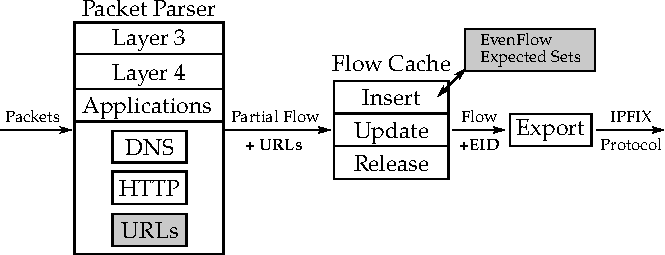
\includegraphics{figures/paper-eventflow/prototype-schema}
    \caption{EventFlow Prototype Schema.}
    \label{fig:eventflow-prototype-schema}
\end{figure}


The FlowMon exporter consists of three main components as shown in Figure~\ref{fig:eventflow-prototype-schema}. The first component is a packet parser. It receives packets from the network and extracts information from a network to application layer of each packet. The extracted information is used to create a partial flow record, which contains all necessary information about the parsed packet such as IP addresses, ports, timestamps, and a byte counter. It also contains application layer information when an application parsing is performed. The partial flow record is passed to the second component of the exporter which is a flow cache. The partial record is either inserted as a new flow record or used to update an existing flow record, which is an aggregation of previous partial flow records. When a flow record expires, it is released from the flow cache to an export component. The purpose of the export component is to convert raw flow records to a flow export protocol format such as NetFlow~\cite{rfc3954} or IPFIX~\cite{rfc7011} and pass the flow records over the network for further processing.

Plugins that extend the FlowMon exporter to process specific application layer protocols, such as DNS or HTTP have access to several parts of the flow creation and export process. Each plugin can request to see the raw packet payload, process it, and add its own information to flow records, such as HTTP Host, Content-Type, or Response Code. Furthermore, the plugins are allowed to provide their own functionality for insert, update, and release methods of the flow cache. Lastly, each plugin defines how the information inserted into flow records is processed by the export component.

The EventFlow prototype is implemented as an application protocol extension. However, it also utilises the data provided by other application plugins. The EventFlow combines information from the DNS and HTTP protocols to detect relations between flows; therefore it requires the DNS and HTTP application plugins to be deployed as well. The prototype extends the packet parser to extract URLs from HTML pages. These URLs are sent together with partial flow record to the flow cache. However, they are used only internally, and they are newer exported in the flow records. When a new flow record is created in the flow cache, the expected sets (see Section~\ref{subsec:eventflow-architecture}) are searched for a match to the new record using DNS, HTTP, and URL information provided in the partial record. If a match is found, the new flow records are assigned an Event ID (8-byte unsigned integer) of the matched record from the expected sets. Otherwise, if no match is found, a new EID is incrementally assigned to the new flow record. After the flow is expired from the cache, the EID is a part of the record and is sent by the export component along with the rest of the flow record.

Using an 8-byte integer for EID and assigning it incrementally to individual events ensures that there are no collisions due to EID overflow in practice. However, an assignment that is individual for each flow probe and persistent over the reboots of the system would be required for a real-world deployment. The EID is assigned only to flows of the HTTP and DNS traffic since it would provide no benefit to other flows as event relation tracking is not implemented for other protocols yet. Moreover, the size of the flows grows only by 8 bytes at maximum, which has a negligible impact on the flow collector disk space requirements.


\subsection{Experimental Evaluation} \label{subsec:eventflow-evaluation}

We evaluate the prototype in two scenarios. First, we assess the functionality of the prototype on a simple example web site. Once we have verified the functionality, we run EventFlow on a packet trace from live network to determine how many flows can be joined to events in real traffic. The IPFIXcol~\cite{Velan-2012-Flow} flow collector is used to collect and process the generated flows. The main advantage of the collector is that it can be easily configured to work with the Event ID element.

We do not evaluate the performance of the prototype in this phase. We are aware of several performance inefficiencies that need to be solved before any valuable results can be measured. For example, one of the most expensive parts of the prototype is the management of sets of expected records. We expect that changing the underlying data structures will significantly improve the performance.

\subsubsection{Functional Evaluation}
For the first scenario, we create a simple website with two pages, each linking the other page, displaying an image, and referencing a different JavaScript library. The evaluation proceeds as follows. We request the first page in a browser and few seconds after it loads we follow the link to the other page. The packet trace of these actions is recorded and processed by the EventFlow prototype, and the resulting flows are collected by the IPFIXcol.

We expect to see a flow record for each of the requests and responses. However, due to the HTTP pipelining the whole communication with the web server hosting the test pages is done using a single connection. Therefore, there is a pair of flows for the accessing the two web pages with the linked images (which were on the same server), two pairs of flows for each off-site JavaScript library, and three pairs of DNS flows for IP address resolution. There are 12 flows created in this test scenario in total. The 12 flows are divided into two events by the EventFlow prototype. The first event contains flows for the two DNS requests, HTTP communication with the web server and download of the first JavaScript library. The second event does not contain an HTTP flow due to the HTTP pipelining but contains the DNS request and the subsequent download of the second JavaScript library.

The functional evaluation shows that the prototype correctly recognises related flows and labels them as a part of the same event. The flow exporter can be extended to handle HTTP pipelining by creating new flow record for each pipelined request. Such extension would make the measurement more accurate, and we plan to deploy it in the future.

\subsubsection{Real Traffic Evaluation}

\begin{table}[!tb]
    \caption{Real Traffic Evaluation Statistics.}
    \centering
    \renewcommand{\arraystretch}{1.1}
    \begin{tabular}{|l|r|} \hline
        \textit{Total Flows} & 613953 \\ \hline
        \textit{HTTP Requests} & 33294  \\  \hline
        \textit{HTTP Responses} & 49753  \\  \hline
        \textit{DNS Requests} & 197926  \\  \hline
        \textit{DNS Responses} & 224588  \\  \hline
        \textit{Events with $>$ 1 Flow} & 28064  \\  \hline
        \textit{Flows in Events with $>$ 1 Flow} & 55881  \\  \hline
        \textit{All Events} & 388749 \\  \hline
        \textit{Flows in All Events} & 418671 \\  \hline
    \end{tabular}
    \label{tab:eventflow-stats}
\end{table}

The purpose of the real traffic test is to determine how many flows can be joined into events. We collect a short (approximately one minute) trace of 10 million packets from an ISP network on ports 53 and 80 which are likely to be DNS and HTTP packets. Table~\ref{tab:eventflow-stats} shows statistics that describe the packet trace as well as the results of the evaluation. We can see that from the total number of more than 600 thousand flows more than 400 thousand are part of events. Furthermore, over 55 thousand flows are part of events which contain more than one flow. Therefore, we can conclude that more than 10\,\% of observed HTTP and DNS flows are recognised as a part of more complex events by the EventFlow prototype.

The number of flows in complex events is not as high as might be expected given the large number of HTTP and DNS requests and responses. We believe that this is caused by a quite short time window of our trace, which is likely to have captured a large number of separate responses and requests. Moreover, we believe that better results can be achieved by fine-tuning the timeout of the records in the expected sets of the EventFlow prototype.


\subsection{Conclusions} \label{subsec:eventflow-conclusions}

We have presented an EventFlow monitoring architecture that allows keeping track of relations between HTTP and DNS application flows, which can be used to simplify behavioural analysis of network traffic, improve network threat detection and network traffic classification. The changes to existing flow monitoring architecture are negligible, which facilitates wide deployment. The relation between flows is encoded as an 8-byte unsigned integer called Event ID which is shared by the related flows. The proposed architecture can be further extended to handle more complex HTTP communication, such as redirection return codes.

A prototype of EventFlow plugin for the FlowMon flow exporter has been evaluated on a trace of 10 million packets. We showed that more than 10\,\% of observed HTTP and DNS flows are recognised as a part of more complex events by our prototype. We believe that this result will improve on longer packet trace as well as with more accurate settings of the prototype. Prospective improvements to the prototype as well as its more detailed evaluation, including a performance evaluation, are left for a future work.

We believe that the network analysis will benefit from the supplemental information about flow relations. Our work has shown that it is possible to acquire such information without a significant impact on an existing monitoring architecture and that it is possible to extend the flow monitoring to trace relations of other application protocols.


\section{MetaFlow}\label{sec:metaflow}

The MetaFlow concept aims to provide support for capturing relations between flows observed in encapsulated traffic, such as tunnels. The widely used approach for monitoring encapsulated traffic is to combine flow keys of different layers to create a new flow key. This flow key splits the flow containing the encapsulated traffic into multiple flows based on the encapsulated traffic. An example of this approach is shown in Figure~\ref{fig:metaflow}.

\begin{figure}[!tb]
    \centering 
    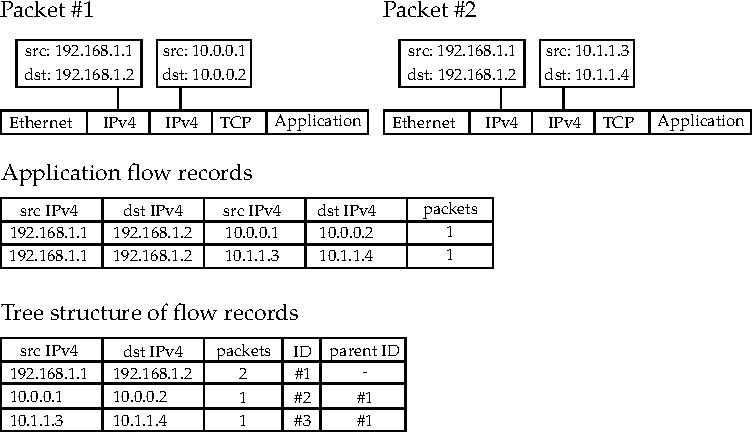
\includegraphics{figures/c07/metaflow}
    \caption{MetaFlow Tree Structure.}
    \label{fig:metaflow}
\end{figure}

We propose to use a more generic approach to handle the encapsulated traffic. In our approach, when an encapsulated traffic is encountered, each layer is treated as a separate flow. Therefore, when a tunnel contains two different communications, we create three different flows. To ensure that the relation between the encapsulation layers is preserved, each flow contains \emph{ID} and \emph{Parent ID} elements, as shown in Figure~\ref{fig:metaflow}. Therefore, the encapsulated traffic is represented by a tree structure.

The main benefit of the MetaFlow approach is that the structure of flows remains the same for an arbitrary number of encapsulation layers. Current flow exporters usually store only the innermost and outermost layers while ignoring any intermediate layers altogether. By providing a uniform way to describe more complex packet structures, we can gain more information about the traffic. Moreover, the flow records are easier to process as well. For example, it is simple to select all encapsulated flows by selecting all flows with non-empty \emph{Parent ID}.

The uniform description allows running queries and algorithms on encapsulated traffic with no additional changes in the flow data processing. When the encapsulated traffic is monitored nowadays, both sets of IP addresses that are present in flow records must be handled, which creates complicated conditions in the code. However, by simplifying the flow records, this problem is removed. Another advantage of the simplified flow records it the lowered number of templates created during flow export. Currently, each layer of encapsulation creates a whole new set of templates that match the templates generated without encapsulation. For example, IPv4 packets with ICMP, UDP, and TCP transport layer protocols usually create three different templates. When the IPv4 header encapsulates another IPv4 protocol header, three new templates are created for ICMP, UDP, and TCP protocols observed in the encapsulated traffic. Handling of a large number of templates is inefficient both for flow export and flow data processing. The MetaFlow removes this inefficiency as no new templates are added at all in this scenario.

To implement MetaFlow, changes would need to be made both to flow data creation and flow data processing. The main modification is that each flow needs to have a unique \emph{ID}. There are several options for generating a unique identifier for each flow during the flow creation process:
\begin{itemize}
    \item A sequence number,
    \item a high-precision timestamp,
    \item a hash.
\end{itemize}

Using a sequence number is fine as long as only a single flow cache is utilised. Shared sequence number means unnecessary synchronisation point for multiple flow caches, which could decrease performance. Moreover, when the exporter is restarted, the numbers would have to continue in the sequence, which is hard to implement in case of sudden reboots and crashes. It the sequence was restarted, the flow collector would have to detect it and renumber the flows, which would lead to consistency problems.

Using high-precision timestamps is fine as long as each consecutive packets are guaranteed to receive different timestamp. If this condition is met, each flow can simply get its start timestamp as its \emph{ID}. For example, the precision needed for 100\,Gbps network would need to be in nanoseconds.

Another option is to utilise the same hash that is used to identify the flow during the flow creation process. However, the hash needs to change when the flow is exported and never be used again. Therefore, the best option seems to be using high-precision timestamps. When they are not available, a combination of hash mixed together with a timestamp will suffice.

Once a flow is received by a collector, the \emph{ID} and \emph{Parent ID} needs to be used together with an identification of the flow exporter. Otherwise, the flows might be mixed as there is no guarantee that each exported generates unique identifiers.

The implementation of flow data processing would need to be reviewed to ensure compatibility with the MetaFlow concept. However, we expect that only minimal changes to flow processing algorithms would need to be done to handle the new format.

\section{Application Events and Flow}\label{sec:app-events}

A concept similar to MetaFlow can be applied to application events as well. Currently, an application flow can be split into multiple flows based on the application content, e.g. multiple HTTP requests on a single connection in separate flows. The result is the same as for encapsulated traffic. Statistical properties of basic flows are broken by the application layer. Moreover, mixing together basic flow which focuses on network and transport layers and the application data forces too narrow view of the available data. We propose to separate application layer data from the basic flow records in the same fashion as MetaFlow separates encapsulated layers from the parent flow. This would effectively decouple application events from the basic flows.

There are three major benefits to our proposal. Firstly, the basic flows remain untouched whatever the application layer information is. This allows detection and statistical methods to rely on the properties of the basic flows without taking into account possible transformation by the application layer. Moreover, when the application layer is not necessary for flow processing, it can easily be filtered out without modification of each flow record. This might lead to major performance benefits for the flow data processing systems.

Secondly, the flow exporter does not have to hold the application information in the flow cache. The flow cache can be implemented efficiently with small flow records without variable fields and dynamically allocated memory. The processing of application events would be moved to packet processing. If the event has no duration, it can be exported directly without delay. We assume that the associated flow identifier is known from the time the flow records is created in the flow cache and therefore can be assigned to the application event at any time. If the application event has a duration, the packet parser must store it in an appropriate application-specific cache until the time it is completed and exported. We expect this mode of data processing at the flow exporter to be significantly more effective than the current mode which holds all application data in flow cache together with the flow records.

The last major advantage is in the processing of the application events. Since each application event is exported separately, the number of templates is significantly reduced. Instead of many combinations of network, transport and application layers, we only have combinations of network and transport layers and then separate templates for application events. Moreover, this separation can simplify the processing of the flows as well. For example, when a detection module requires only data from HTTP and DNS protocols, it can easily select only the two templates to work with. 

The proposed approach has one notable disadvantage. The flow processing systems are going to receive application events before the flow records expire. This might cause them to buffer the data and wait for the flow records. However, basic information about each flow, such as IP addresses, transport protocol, and port numbers can be included in the application event messages as well. This should facilitate unhindered processing of the flow events while the flow records are being aggregated. Moreover, detection methods using application events could react much faster than those utilising application flow records.

Since the application data are effectively decoupled from the basic flows, we can quite easily inject data from another source, such as application logs to the data stream. The injected data can share the same template with the application events, which would facilitate the shared processing. Moreover, based on timestamps and network information, the injected data could be attached to the basic flows as well. There are several reasons to do this. Firstly, the logs can provide ground truth for the application layer data. Secondly, having a single system processing all available data from the network and host systems helps to improve quality of data and accuracy of various detection algorithms. Lastly, using a single system to process data from multiple sources reduces management and running costs.

\section{Summary}\label{sec:ng-summary}

We have proposed several novel concepts for application flow monitoring in this chapter. Each of our proposals could be implemented separately; however, we believe that a combination of all proposed approaches is not only possible but would provide greatest benefits for the application flow monitoring.

The first proposed concept has been EventFlow. It is an extension of the flow measurement which allows preserving relations between HTTP and DNS application flows that are a part of single user action, most typically browsing a web page. We have described an architecture of the EventFlow extension and its limitations. A prototype implementation of the EventFlow has been introduced and evaluated on a packet trace from an ISP network. We have shown that a significant number of flow records can be recognised as a part of a single user action.

MetaFlow has been proposed as an approach to monitoring of encapsulated traffic. We have argued that the current practice of extending flow records with information from each layer is not flexible and has several disadvantages. MetaFlow aims to create a hierarchy of encapsulated flows so that each flow is able to retain a simple structure while the information about the relations between flows is preserved. We have also discussed how to create a unique flow identifier, which is necessary for building the MetaFlow tree structure.

The last proposal has expanded the MetaFlow concept to application layer events. By decoupling application events from basic flow records, we can significantly simplify both flow creation process and flow data processing systems. Moreover, it allows us to solve issues produced by the forceful splitting of flows based on application payload. We believe that separating application events from basic flow monitoring is the future of application flow monitoring. Moreover, this approach provides new opportunities for novel research not only for flow monitoring but also for flow data processing systems.